\subsection{Magnetic Fields and Magnetic Forces} 

%\DTMnewdatestyle{dateupdated}{〈definition 〉

Answers to M\Alph{subsection} problems are on page \pageref{magnetism_prob_answers}.  \textbf{\textcolor{red}{Updated \DTMnow.}}


%--------------------------------------------------------------------------------------------------------------
\begin{Exercise}
A current $I$ flows in a single, infinitely long wire that is bent at a $90\degree$ angle, as shown in the figure below on the left.  
Find the magnetic field $\vec{B}$ (magnitude and direction) at the point $P$, which is a  distance $y$ above the corner of the wire, as shown below.  
(Hint: Think about this problem the same way as you found $B$ due to a single, straight wire in Lab~\ref{biot_savart_straight_wire} using the Biot-Savart law.  
In that lab, you had a single wire, running from $x=-L/2\text{ to }+L/2$.  
Here, the horizontal part of the bent wire looks exactly like the wire in that lab, except that it runs from $0\text{ to }\infty$.  
For the vertical part of the bent wire, you will need to rethink how to apply the Biot-Savart law, particularly the result of the cross product $\vec{ds} \times \hat{r}$.)
\end{Exercise}
\begin{Answer}
$B=\mu_0 I / 4\pi y$, into the page 
 \end{Answer}

\hspace{\fill}
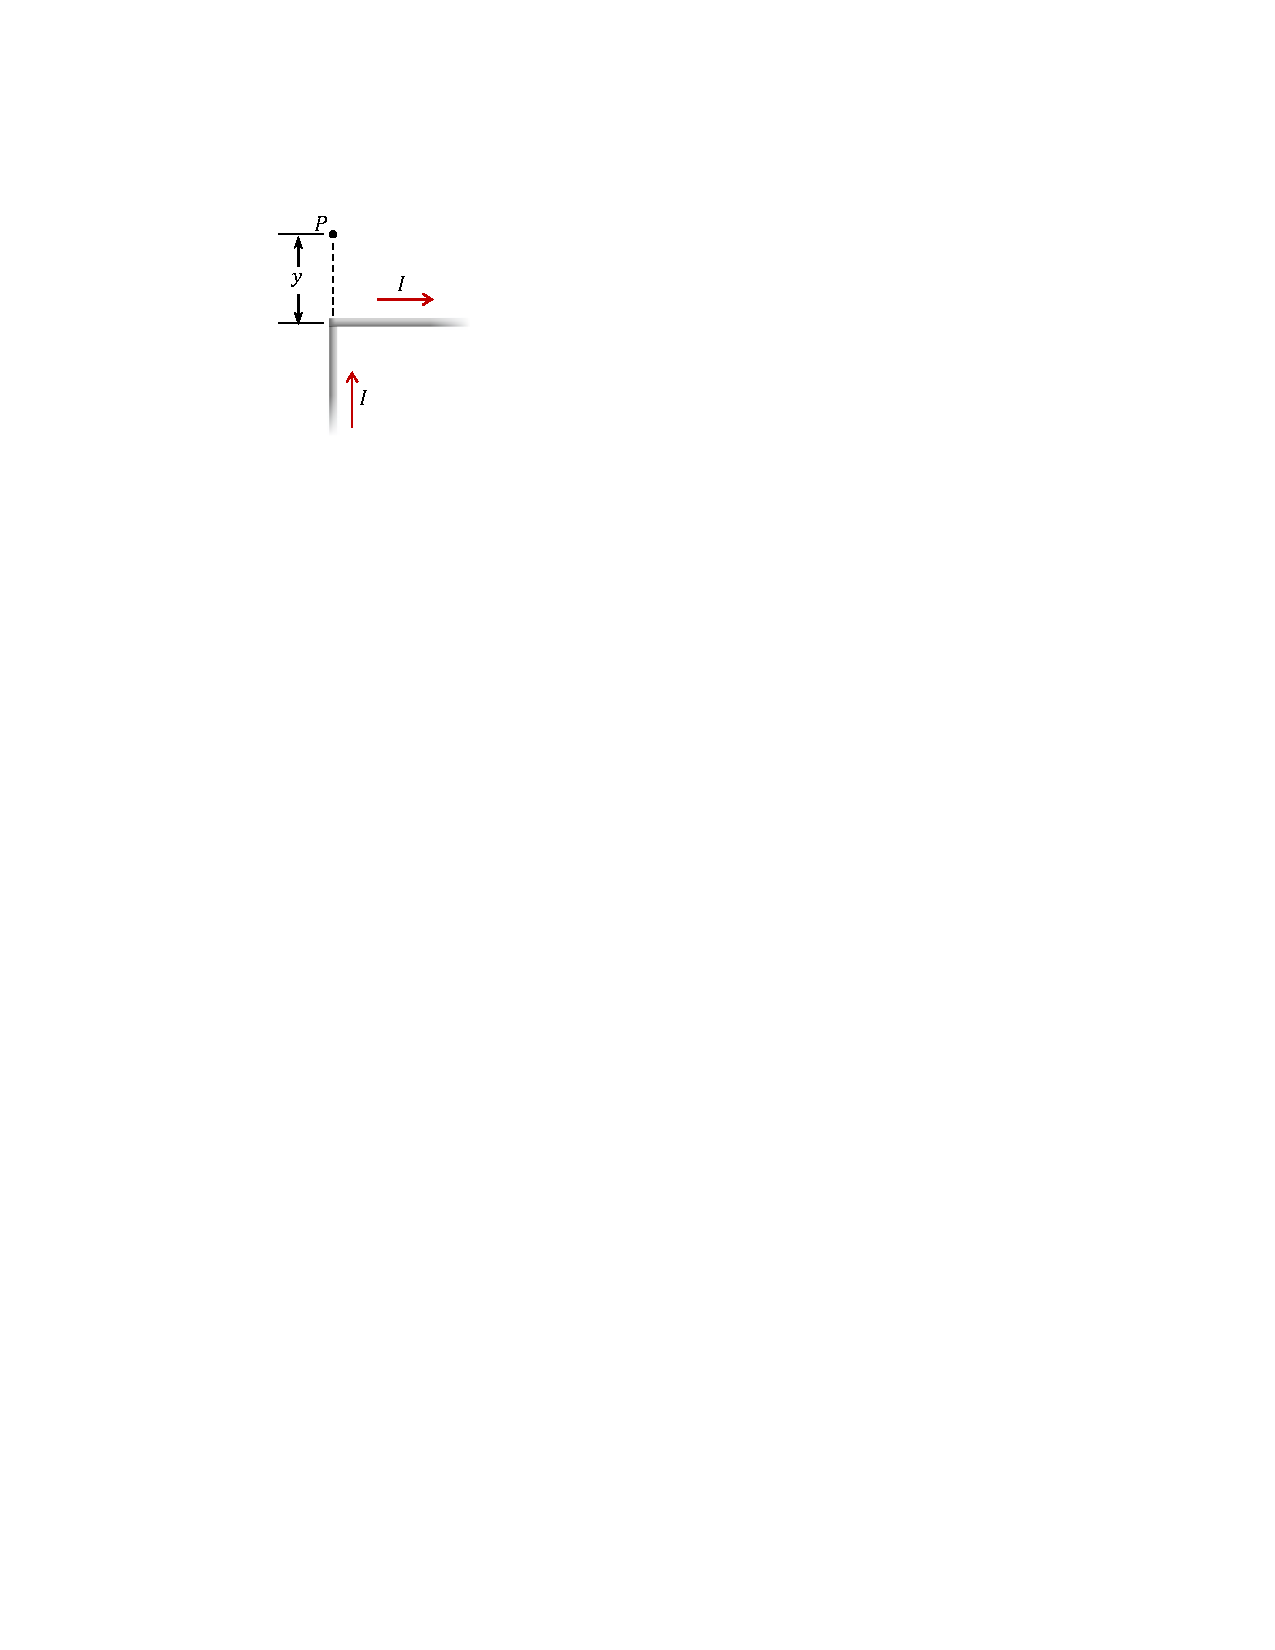
\includegraphics{M_problems/magnetism/right_angle_infinite.pdf}
\hspace{\fill}
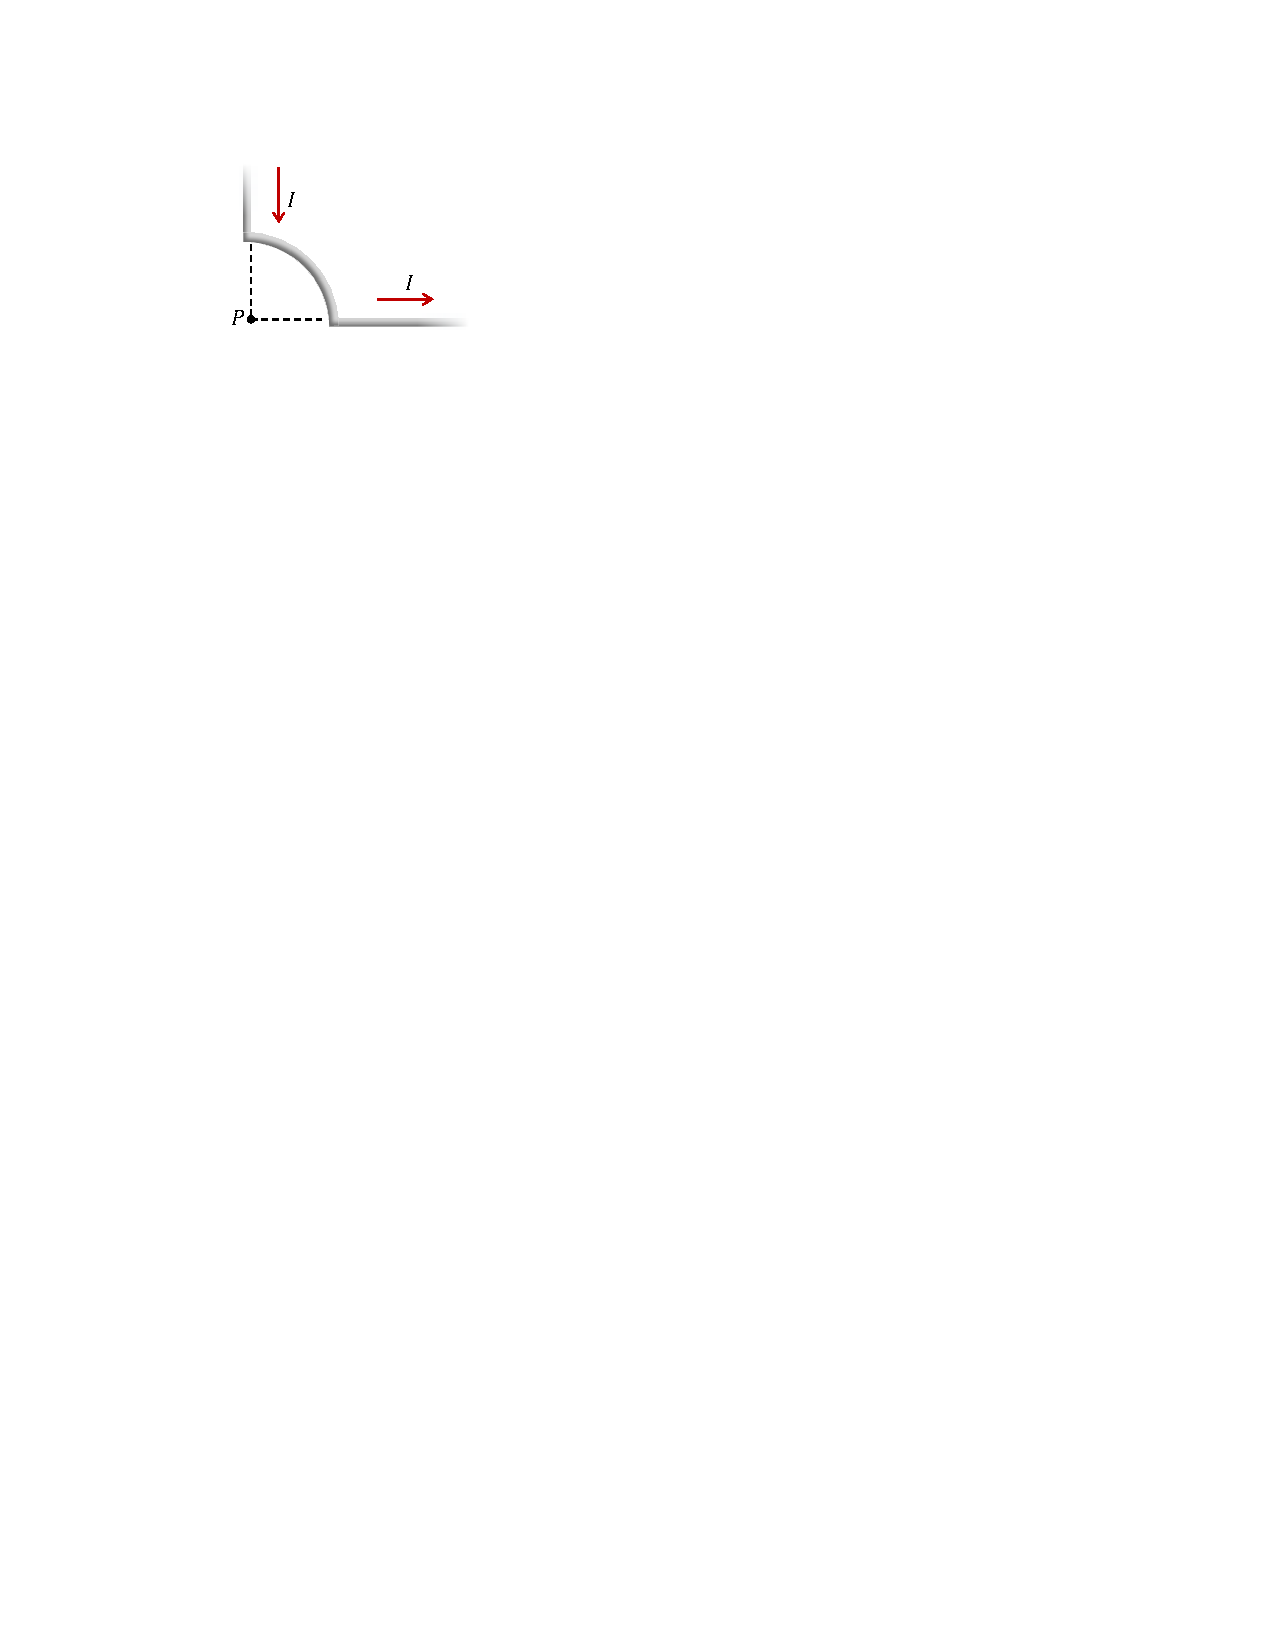
\includegraphics{M_problems/magnetism/quarter_loop_and_infinite.pdf}
\hspace{\fill}

%--------------------------------------------------------------------------------------------------------------
\begin{Exercise}
A single wire carries current $I$ in the path shown, with a straight vertical segment and a straight horizontal segment leading to and from a $90\degree$ circular arc of radius~$R$.  
Find the magnetic field (magnitude and direction) at point~$P$ in the center of the arc.
\end{Exercise}
\begin{Answer}
$B=\mu_0 I / 8R$, into the page
\end{Answer}

%--------------------------------------------------------------------------------------------------------------
\begin{Exercise}
An otherwise straight, infinitely long wire is bent to include a single circular loop of radius $R$, as shown in the figure below.  (a)~What is the direction of the magnetic field at the center of the circular loop?  (b)~What is the magnitude of the magnetic field there?  Hint: in both parts of this problem, you need to account for the magnetic field due to the circular part AND the two straight parts of the wire.
\begin{center}
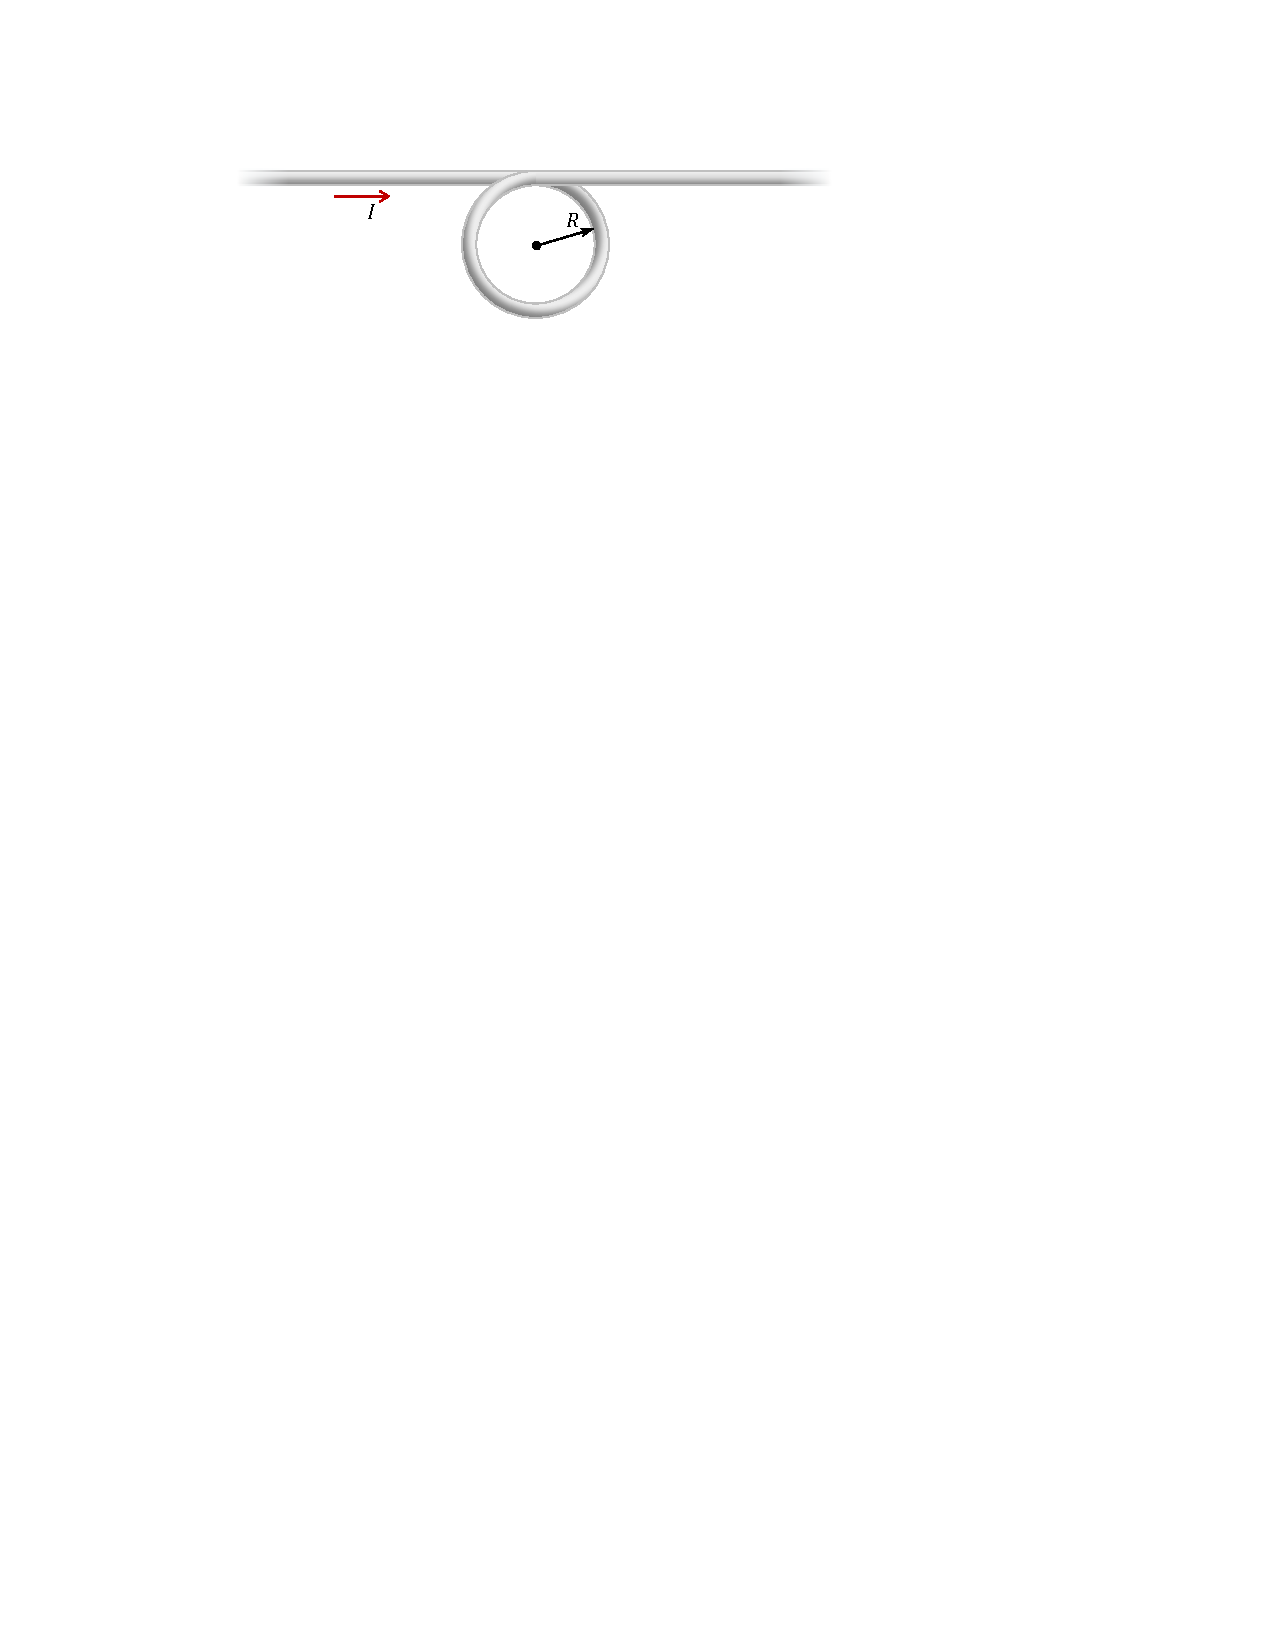
\includegraphics{M_problems/magnetism/straight_wire_with_loop.pdf}
\end{center}
\end{Exercise}
\begin{Answer}
(a) into the page (b) $\displaystyle B=\frac{\mu_0 I}{2R}\left( 1+\frac{1}{\pi}\right)$
\end{Answer}


\figuretoright{0.40}{M_problems/magnetism/three_wires_out_of_page.pdf}{
%--------------------------------------------------------------------------------------------------------------
\begin{Exercise}
The figure to the right shows an end-on view of three very long straight wires, each carrying a current $I=2$~A out of the page.  Taking $a=1.0$~cm, find the magnetic field $\vec{B}$ (magnitude \textit{and} direction) at the points $A$, $B$, and $C$ in the picture.  
\end{Exercise}
\begin{Answer}
point $A:~53.3~\mu$T down (towards bottom of page); \\
point $B:~20.0~\mu$T down; point $C:~\vec{B}=0$
\end{Answer}


%--------------------------------------------------------------------------------------------------------------
\begin{Exercise}
A long, straight wire with a circular cross section of radius $R$ carries a total current $I$, uniformly distributed within it.  (That is, the current density $J$ is the same everywhere inside the wire.)  Find the magnetic field inside the wire, a distance $r$ from the center, where $r<R$. 
\end{Exercise}
\begin{Answer}
$\displaystyle B = \frac{\mu_0 I r}{2\pi R^2}$
\end{Answer}
}

(Hint: use Amp\`ere's law and start with a careful end-on drawing of the circular wire that clearly shows the point at distance $r$, an Amp\`erian loop, and the amount of current $I_\text{enc}$ that is enclosed by the loop.)

\pagebreak[3]
%--------------------------------------------------------------------------------------------------------------
\begin{Exercise}
The picture below on the left shows a cross-section of a ``coaxial cable,'' in which current $I_1$ flows out of the page through the central conductor, and current $I_2$ flows into the page through the outer hollow cylindrical shell.  As with a real cable, the wires are insulated inside and out with rubber insulation.  Taking $I_1=1$~A, $I_2=3$~A, and $d=1$~mm, find magnitude and direction of the magnetic field at both points $a$ and $b$.
\end{Exercise}
\begin{Answer}
(a) 200~$\mu$T, up (towards top of page) (b) 133~$\mu$T down
\end{Answer}

\hspace{\fill}
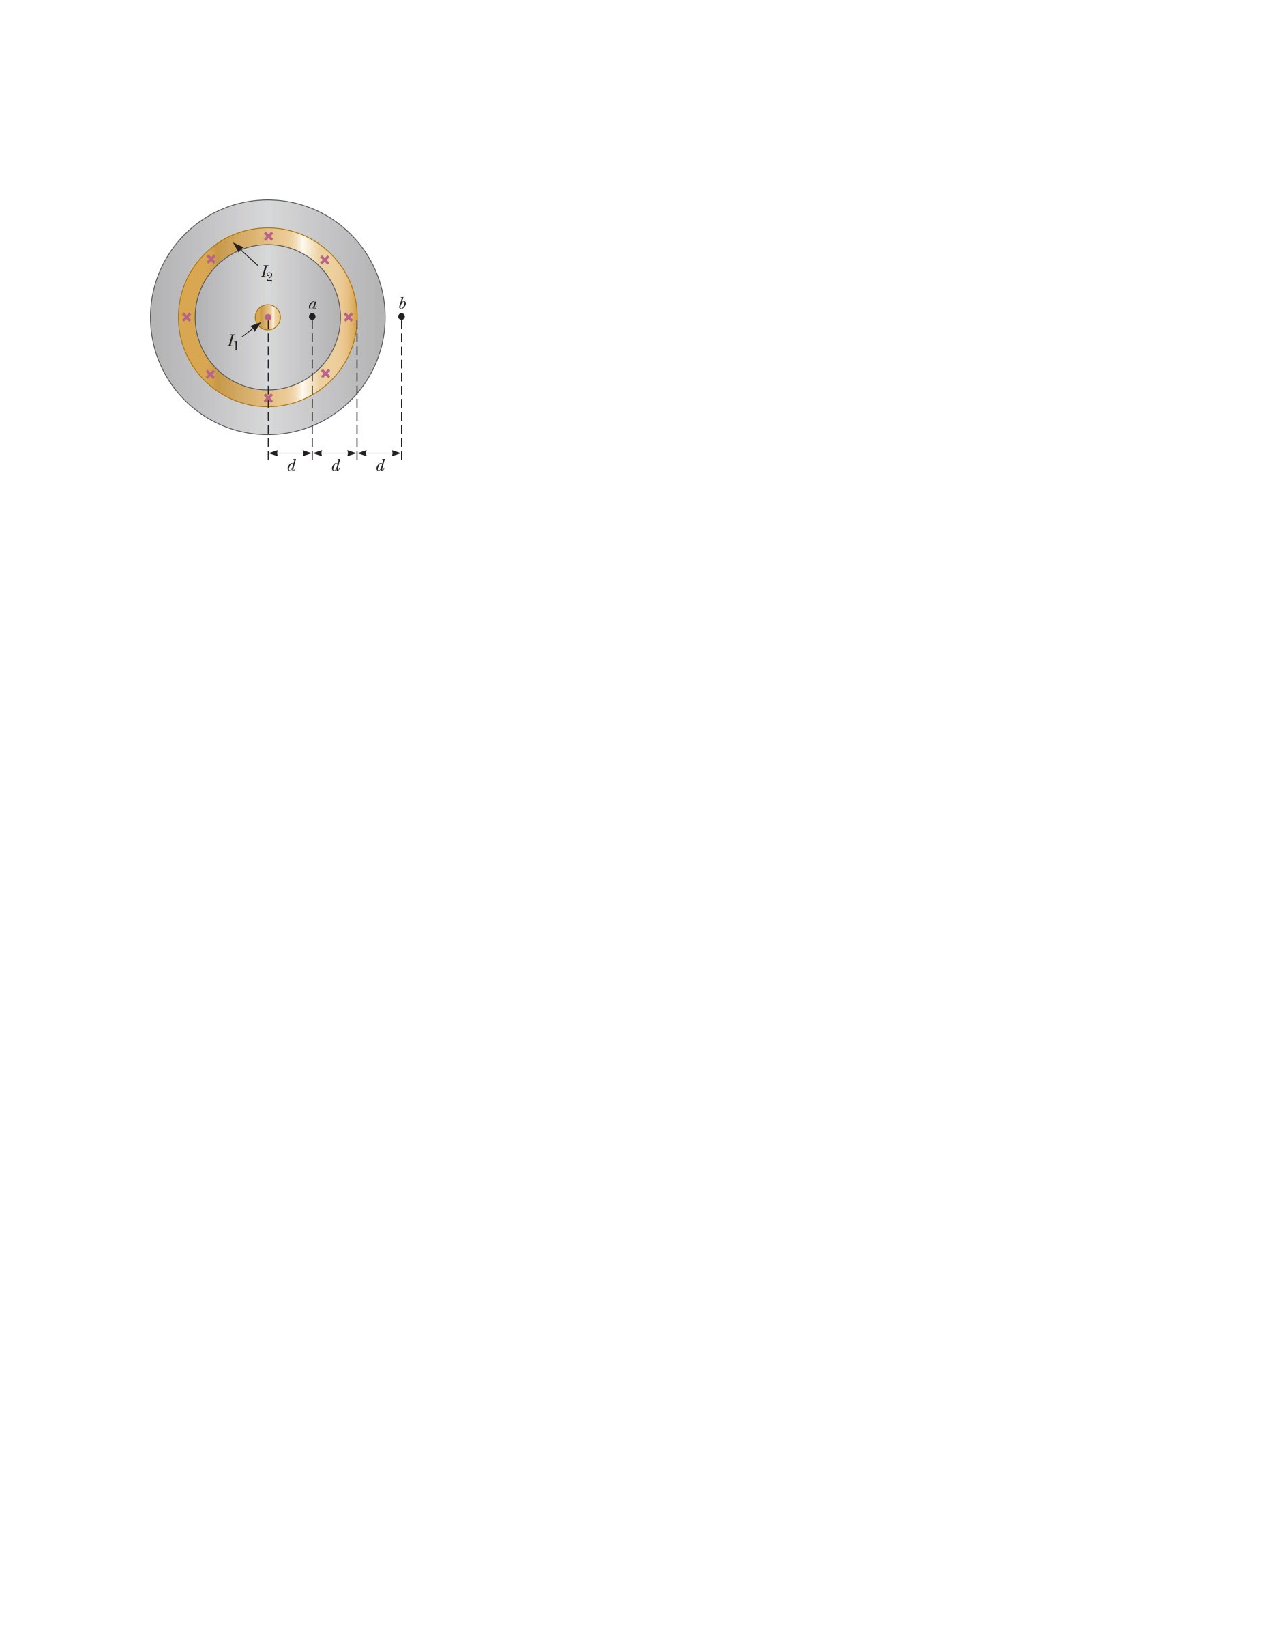
\includegraphics{M_problems/magnetism/coaxial_cable.pdf}
\hspace{\fill}
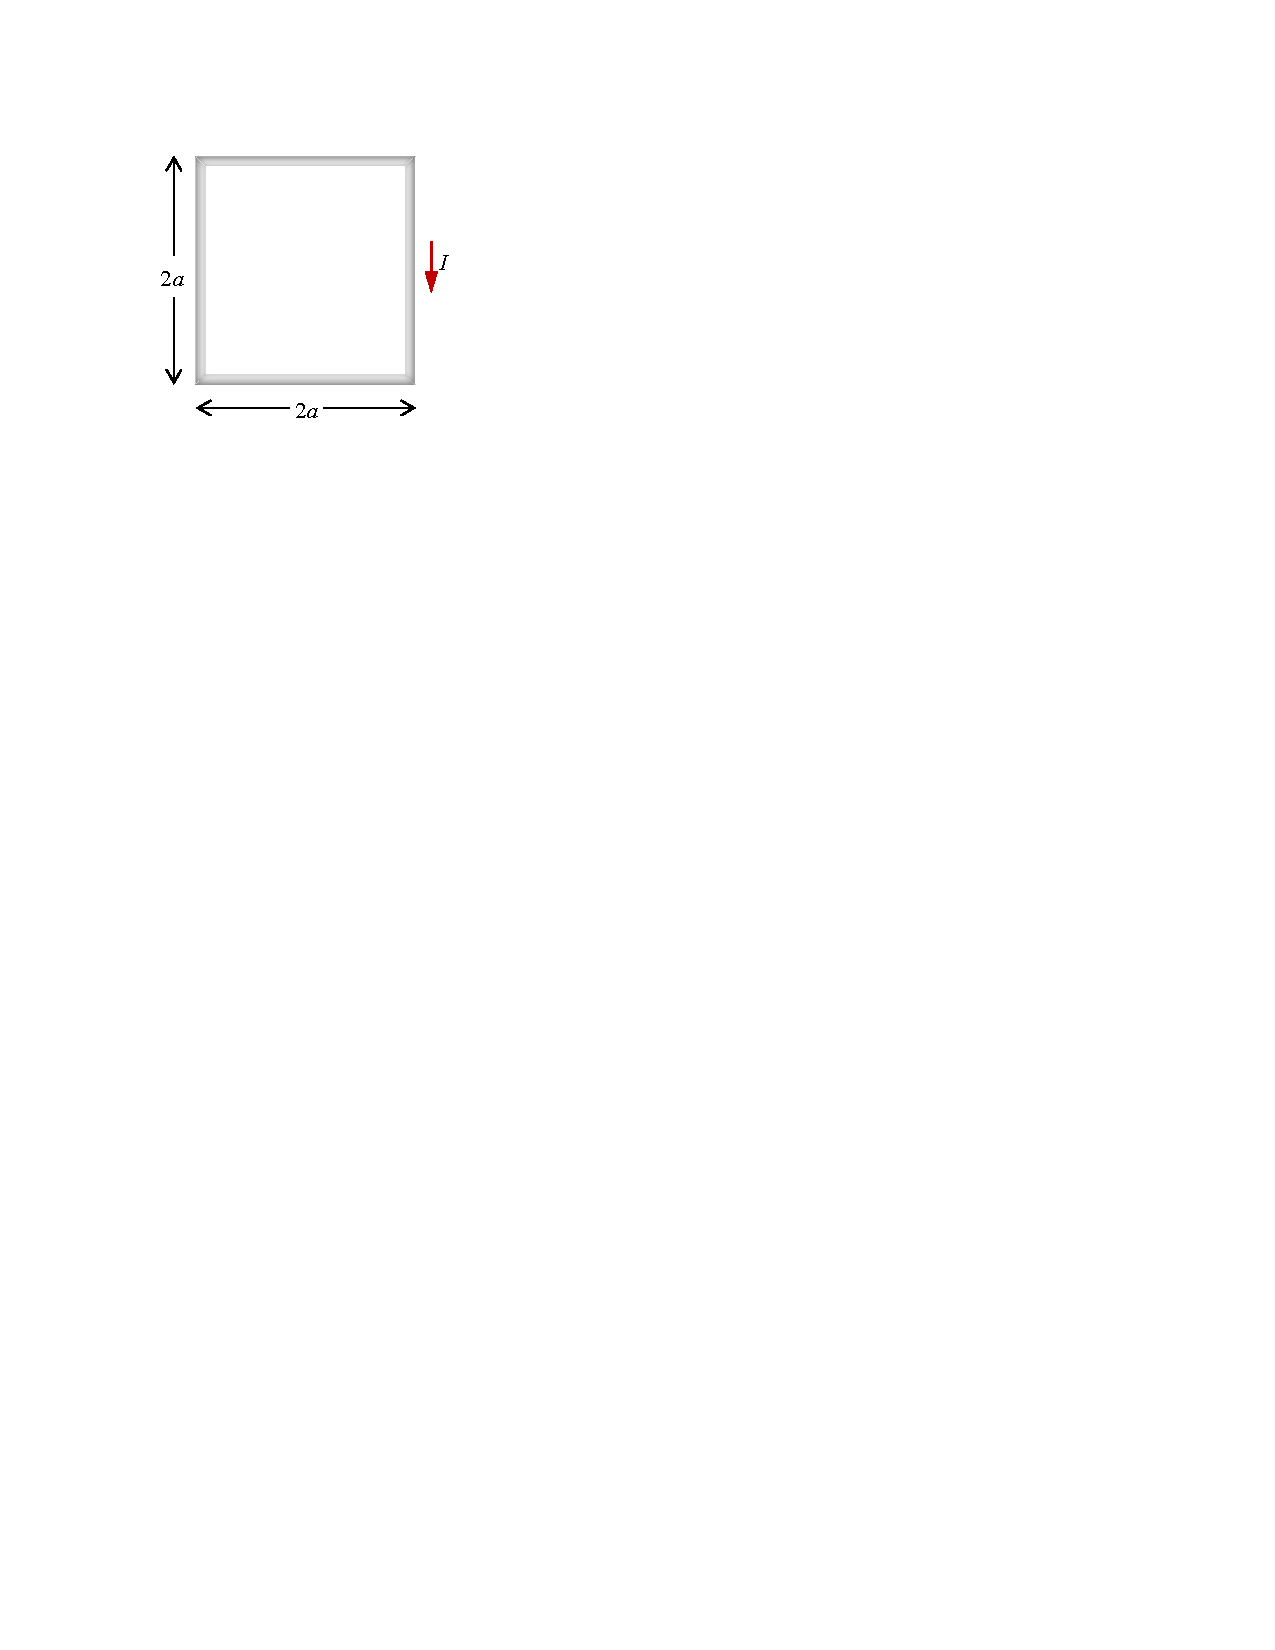
\includegraphics{M_problems/magnetism/square_loop.pdf}
\hspace{\fill}

%--------------------------------------------------------------------------------------------------------------
\begin{Exercise}
A square loop of wire with side length $2a$, pictured above to the right, carries a current $I$.  (a)~Find the magnetic field $\vec{B}$ in the center of the loop.  
For this problem, you can use the result you derived in Step~7 of Lab~\ref{biot_savart_straight_wire}, though you should also be sure you know how to derive that result again if you need to.  (b)~Derive the same result as in part (a) using Amp\`ere's law, or, if it can't be done, explain why not. 
\end{Exercise}
\begin{Answer}
(a) $\displaystyle B = \frac{\sqrt{2}\mu_0 I}{\pi a}$, into the page.
\end{Answer}


%--------------------------------------------------------------------------------------------------------------
\begin{Exercise}
You are already familiar with the magnetic force 

\begin{minipage}[t]{0.74\textwidth}
$$\vec{F}=q\vec{v}\times\vec{B}$$
on a single moving charge $q$, 
and in this problem we'll use that as a starting point to find the force on a current-carrying wire in an external magnetic field $\vec{B}$.
(``External'' means that the field $\vec{B}$ is caused by something \textit{other than} the current in the wire.)  
Our solution will use many of the following familiar quantities: 
$\vec{B}, ~n_e, ~q_e, ~m_e, ~\tau, ~\ell, ~A,$ and $v_\text{drift}.$
\end{minipage}
\begin{minipage}[t]{0.25\textwidth}
\vspace{-0.5in}
\hspace{\fill}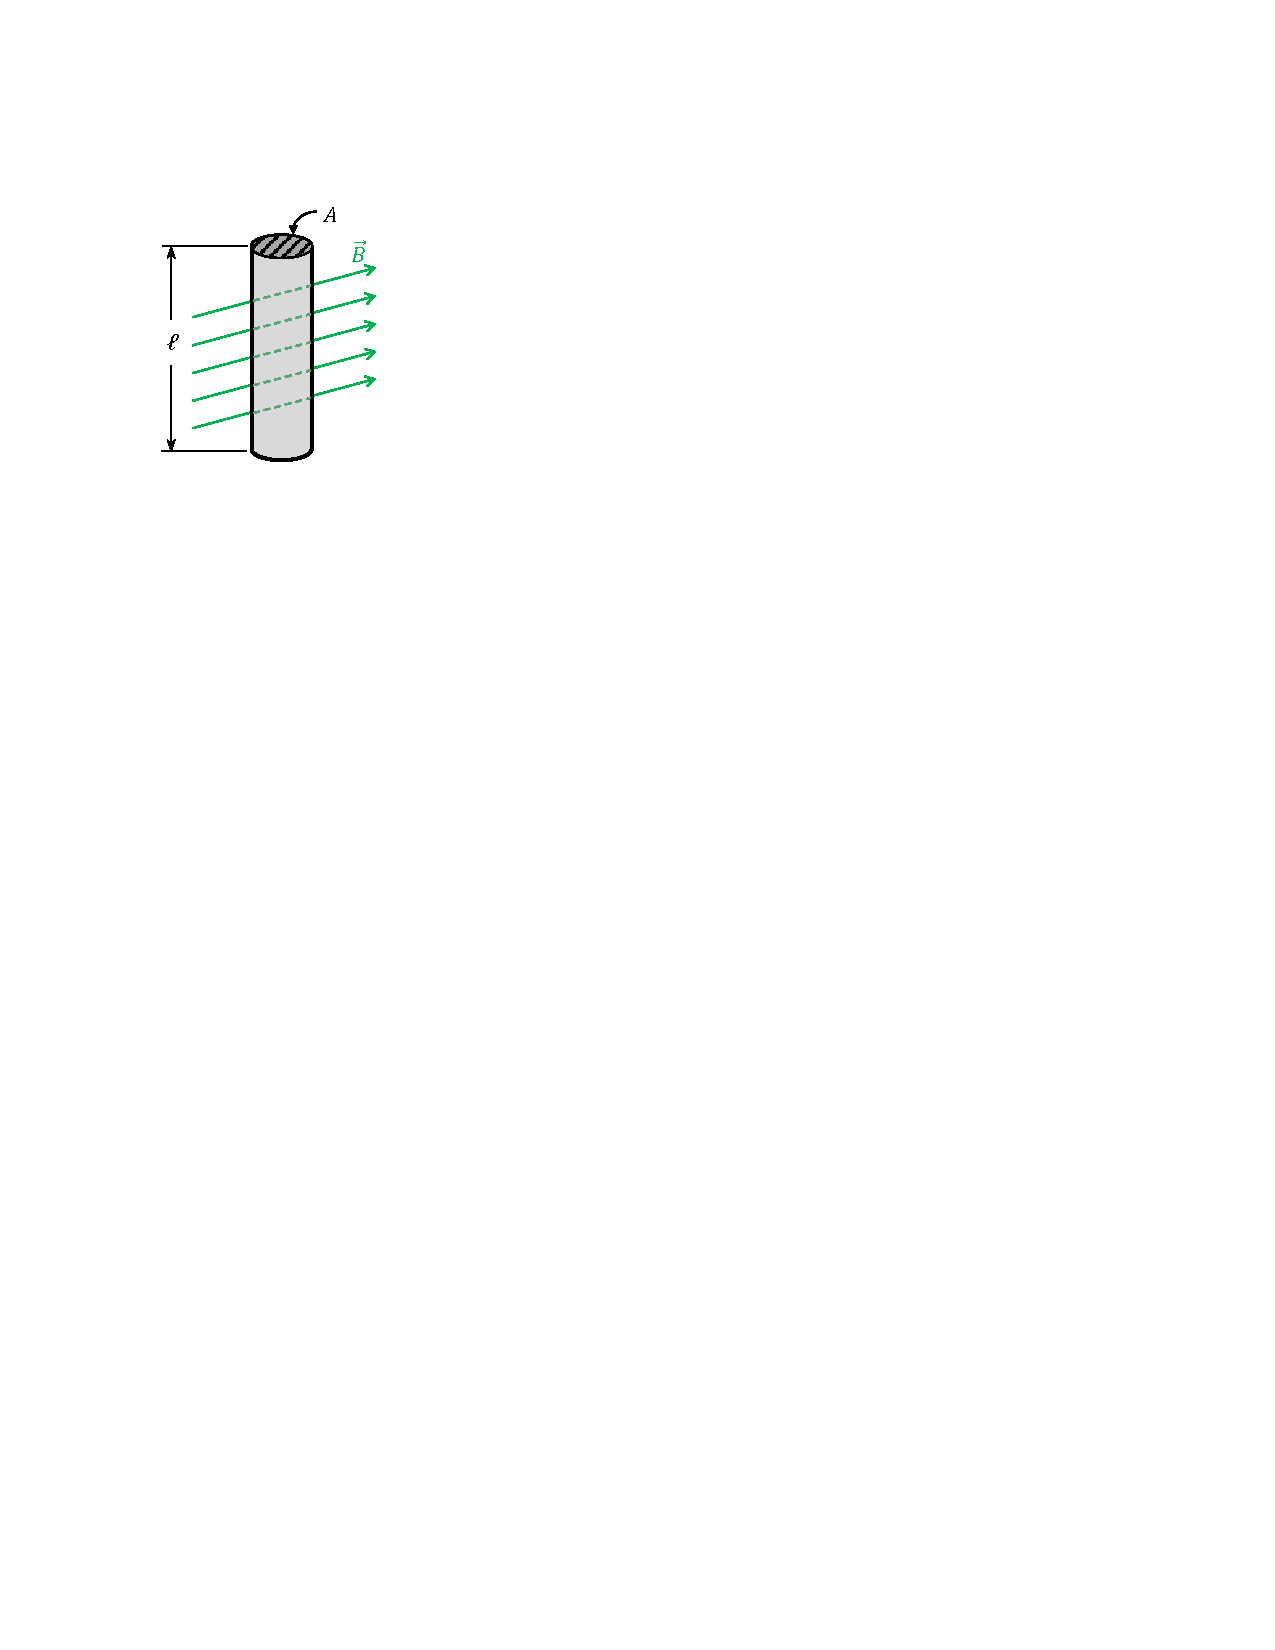
\includegraphics[scale=0.90]{M_problems/magnetism/force_on_wire1.pdf}
\end{minipage}

\begin{enumerate}[labparts,nosep]
\item What is the total number $N$ of moving electrons in the length of wire shown in the figure, using only quantities listed above?
\item What is the average speed of those $N$ electrons in the wire? (Again, from the list above.)
\figuretoright{0.30}[scale=0.9]{M_problems/magnetism/force_on_wire2.pdf}{
\item Write an expression for the total force $\vec{F}$ on all $N$ electrons, using only quantities from the list.
\item The current $I$ in the wire can be written in terms of many of the same variables as your expression for $\vec{F}$ in part~(c).  Make that substitution, to express $\vec{F}$ in terms of $I$ and just two other variables.  (Hint: what is the electron current $i_e$ in terms of the quantities listed above?)
\item Suppose that a not-at-all straight wire is in a non-uniform field.  What is the bit o' force $\vec{F}$ on a short bit o' wire of length $d\vec{s}\,$?
\item And finally, what would be the force $\vec{F}$ on the whole squiggly thing?
}
\end{enumerate}
\end{Exercise}
\begin{Answer}
(d) $\vec{F}=\ell \vec{I} \times \vec{B}$ (f) $\vec{F}=\int I \, d\vec{s} \times \vec{B}$
\end{Answer}

%--------------------------------------------------------------------------------------------------------------
\begin{Exercise}
Goofus and Gallant are working on the review problems for magnetism, and they want to calculate the magnetic field at the center of a current-carrying circular ring of wire of radius $R$.  Gallant uses the Biot-Savart law and correctly calculates $B=\mu_0I/2R$.  Meanwhile, Goofus thinks that he has come up with a great new way to calculate the field by using Amp\`ere's law instead of  the Biot-Savart law.  He draws a dotted circular path with the same radius $R$, perpendicular to the plane of the current-carrying ring and through the ring's center, as shown below.  Using the dotted circular path as his Ampèrian loop, he applies  Amp\`ere's law as follows: 

\begin{minipage}{0.7\textwidth}
\begin{align*}
\oint \vec{B} \cdot d\vec{s} &= \mu_0 I_\text{enc} \\
\implies \oint B \, ds &= \mu_0 I_\text{enc} ~~ (\text{b/c } \vec{B} \perp d\vec{s}) \\
\implies B \oint ds &=  \mu_0 I ~~~~ (\text{b/c } B \text{ const.}) \\
%B(2\pi R)  &=  \mu_0 I  \\
\implies B  &=  \frac {\mu_0 I}{2\pi R}\, , \text{ Q.E.D. by Goofus~~(wrong)} \\
\end{align*}
\end{minipage}
\begin{minipage}{0.29\textwidth}
\vspace{0in}
%\begin{center}

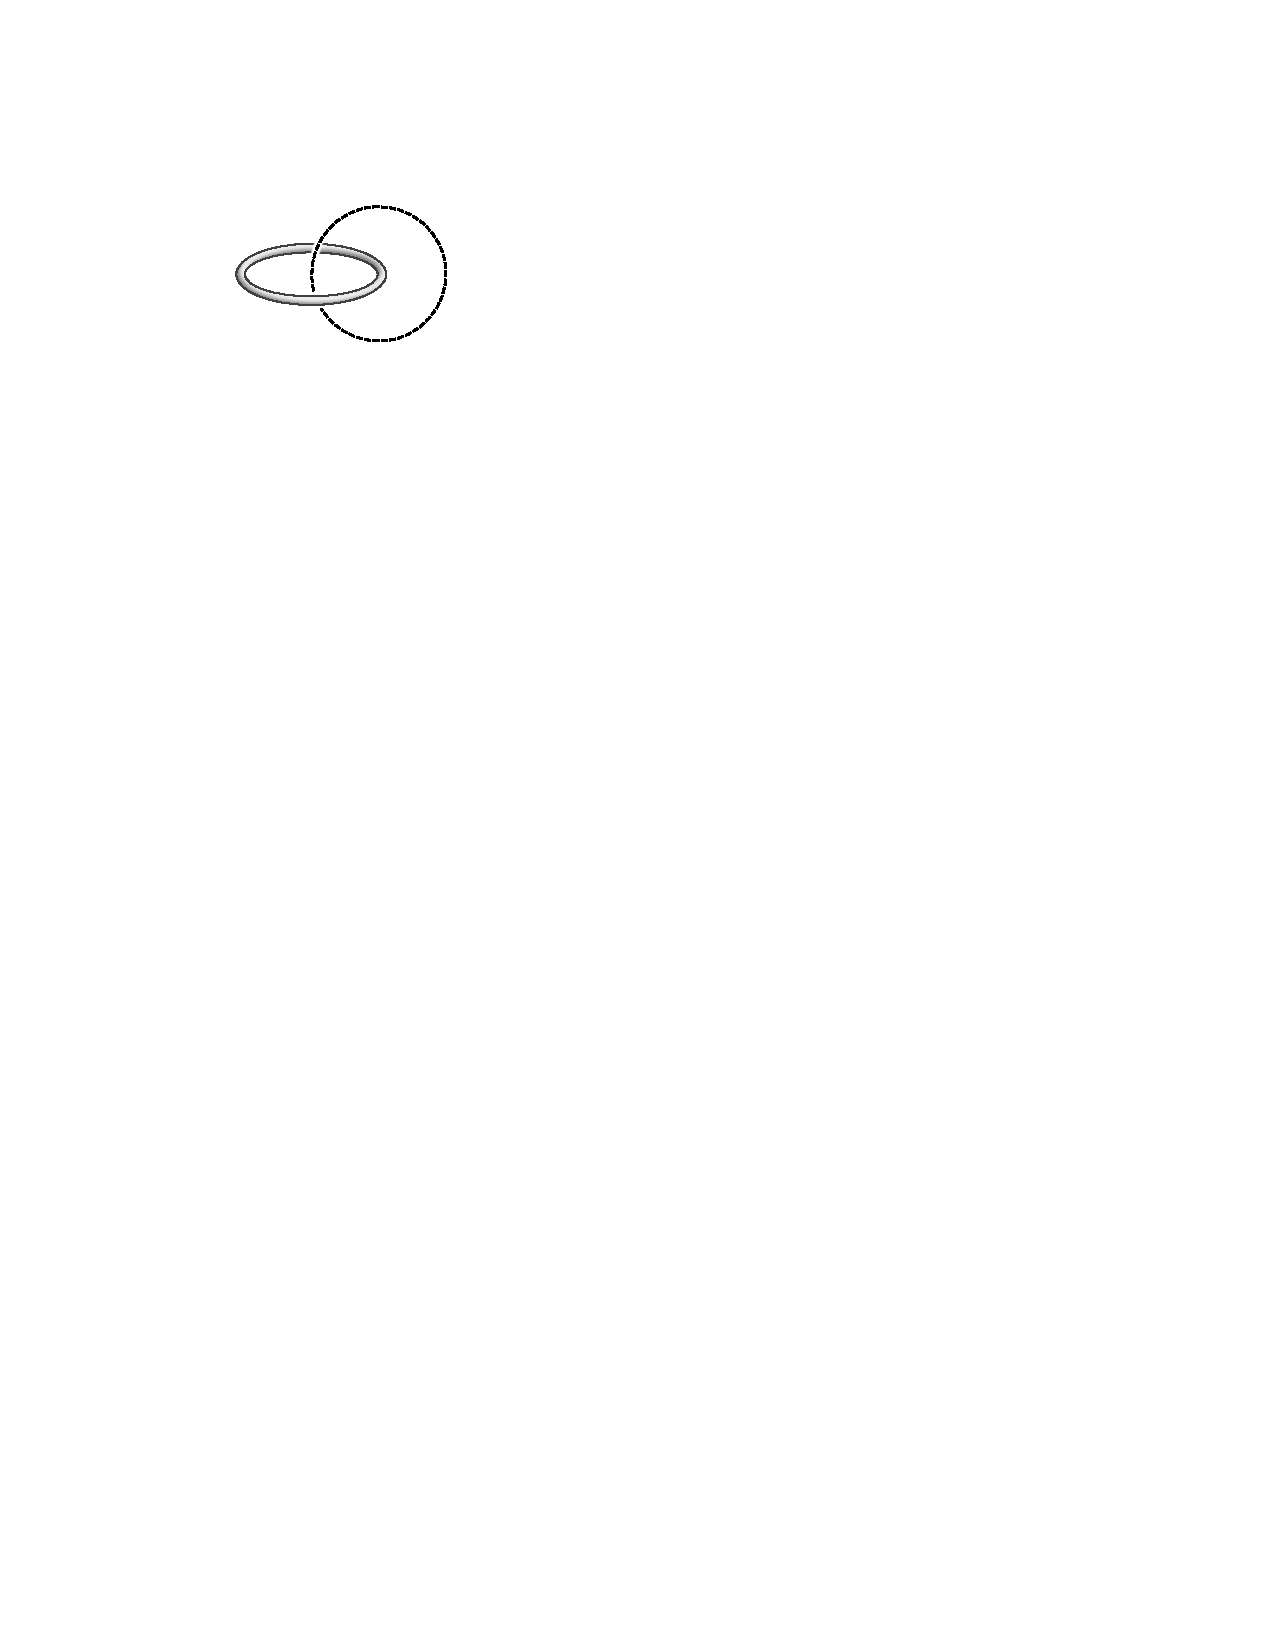
\includegraphics{M_problems/magnetism/goofus_ampere.pdf}
%\end {center}
\end{minipage}


Sadly, Goofus sees that his answer is incorrect by a factor of $\pi$.  
%Gallant sees it too.  
Write a 
%snarky, 
condescending letter from Gallant to Goofus explaining the error in his logic.
\end{Exercise}


%--------------------------------------------------------------------------------------------------------------
\begin{Exercise}
\label{problem_force_on_rectangular_loop}
An infinitely long straight wire carries a current $I_1$. 
A rectangular loop of wire with dimensions $h \times w$, and carrying a current $I_2$, is a distance $d$ away from the straight wire; both are in the plane of the page in the drawing to the right.

\begin{minipage}[t]{0.64\textwidth} 
\begin{enumerate}[labparts]
\item In general, what is the magnetic field a distance $r$ away from an infinitely long, straight wire with current $I$? 
\item Find the direction of the magnetic force on each of the four legs of the rectangular loop.  
\item Find the magnitude of the magnetic force of $I_1$ on only the closest leg of the rectangle. 
\item Find the magnitude of the net force of the straight wire on the rectangular loop.
\end{enumerate}  
Note: the way to think about this problem is that the current in one of these wires causes a magnetic field, and the other wire feels a force due to that field.  In principle, you can either: 
\end{minipage}
\begin{minipage}[t]{0.35\textwidth} 
\vspace{-0.20in}
\hspace{\fill}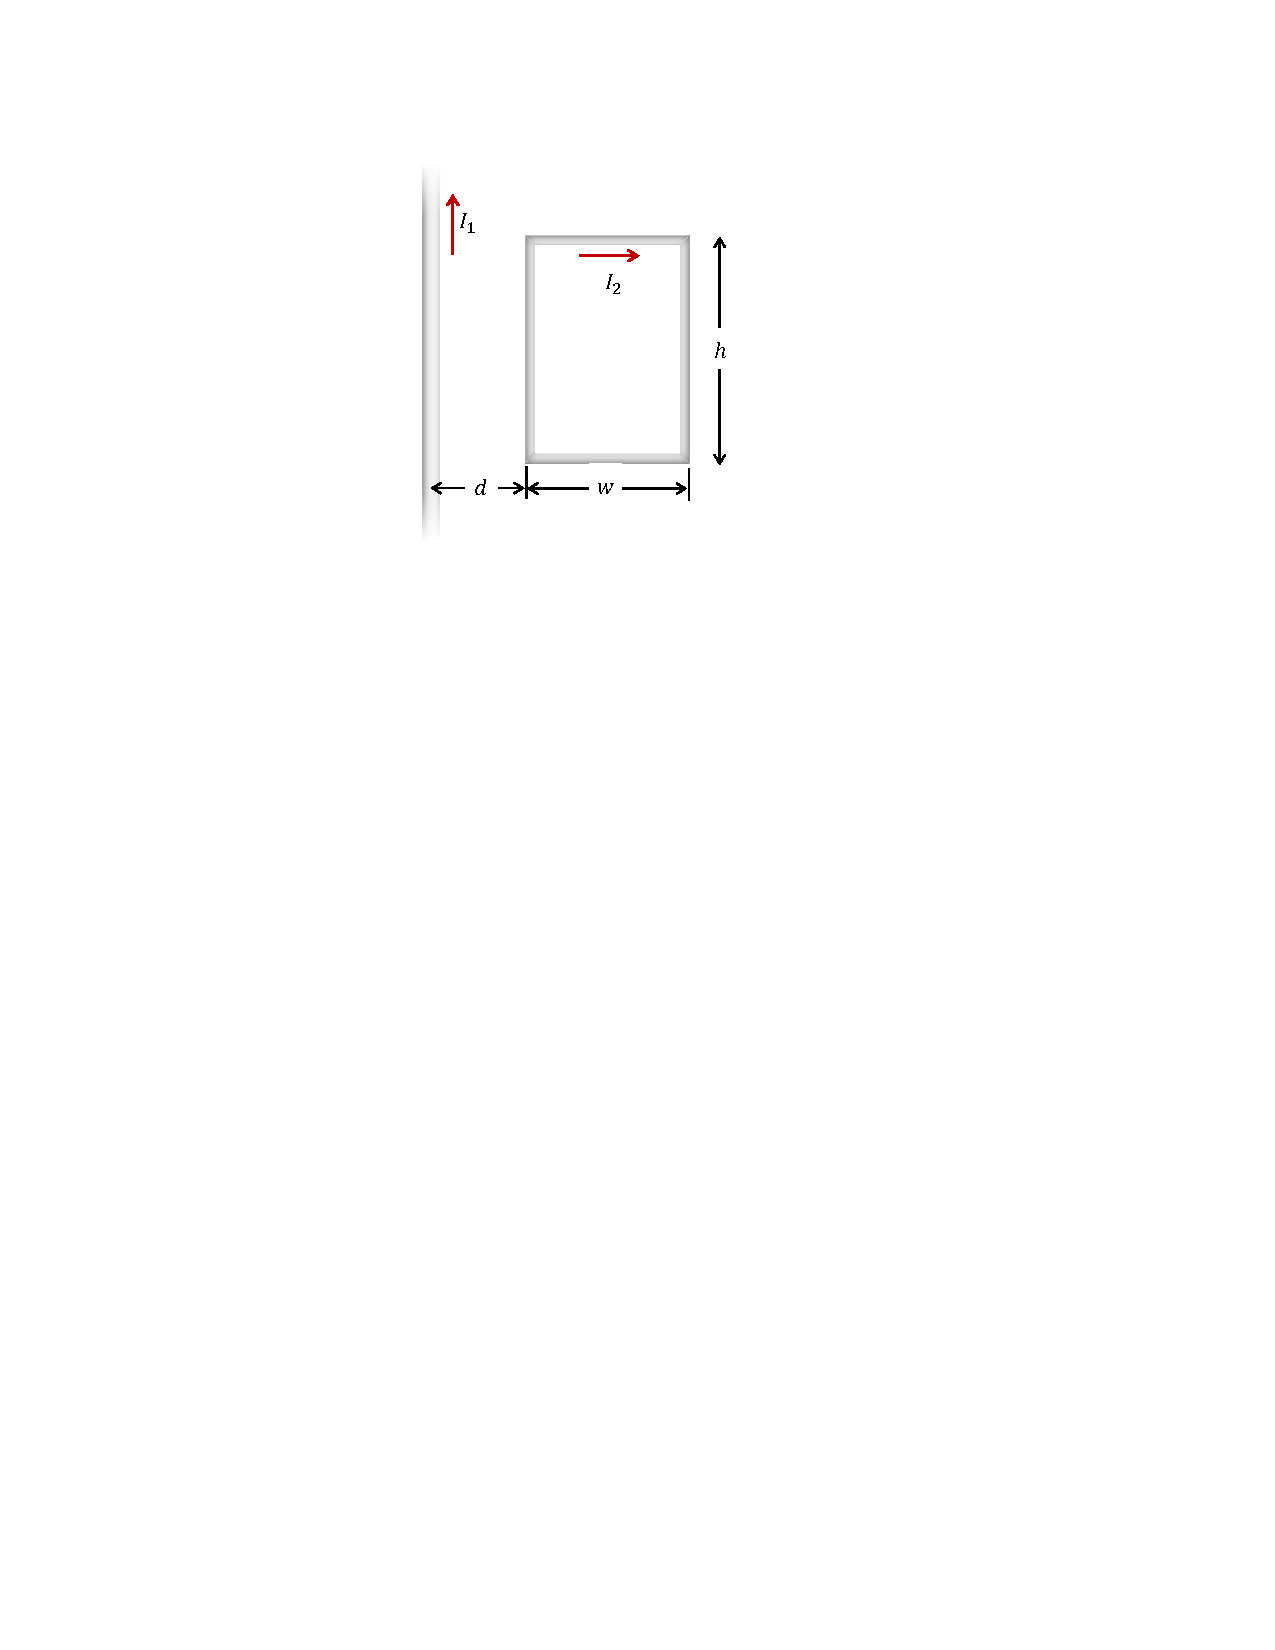
\includegraphics[scale=0.93]{M_problems/magnetism/force_on_rectangular_loop.pdf}
\vspace{-0.20in}
\end{minipage}
\begin{itemize}[nosep]
\item find the field due to $I_1$, then find the force on the wires with $I_2$ due to that field, or 
\item find the field due to $I_2$, then find the force on the wire with $I_1$ due to that field. 
\end{itemize}
One of those two options is much easier than the other; in fact, the other one is disastrous!
\end{Exercise}
\begin{Answer}
(b) All legs are pushed away from center of rectangle.
(c) $\displaystyle F=\frac{\mu_0 I_1 I_2 h}{ 2\pi d} $
(d) $\displaystyle F=\frac{\mu_0 I_1 I_2 hw}{ 2\pi d(d+w)}$
\end{Answer}


%--------------------------------------------------------------------------------------------------------------
\begin{Exercise}
For the situation in problem~\ref{problem_force_on_rectangular_loop}, calculate the magnitude of the force on ONLY the top, horizontal leg of the rectangle carrying current $I_2$.  Hint: start by writing an expression for the infinitesimal force on a tiny bit of that wire of length $dx$. 
\end{Exercise}
\begin{Answer}
$\displaystyle F = \frac{\mu_0 I_1 I_2}{2\pi} \ln \left( \frac{a+c}{c} \right)$
\end{Answer}

%--------------------------------------------------------------------------------------------------------------
\begin{Exercise}
Two students are determining the mass of an electron by doing the same laboratory that you did in class.  They take the following data:
\begin{itemize}[nosep]
\item Current in Helmholtz coils $I=1.45$ amps (multimeter readings are $\pm 0.5\%$).
\item Radius of coils $a=15.0\pm 0.1$ cm.
\item Number of coils $N=130$ exactly.
\item Accelerating voltage $V=184$ volts.
\item Radius of circular path: $r=4.1\pm 0.1$ cm.
\end{itemize}
\begin{enumerate}[labparts,nosep]
\item What is the magnetic field $B$ at the center of the coils?  
\item What is the uncertainty in the magnetic field?  
\item What value should they report for the mass of the electron $m_e$?  
\item What is the uncertainty in $m_e$ due to only the uncertainty in $r$? 
\item What is the uncertainty in $m_e$ due to all sources of uncertainty?  
\item Write an expression for $m_e$ involving only quantities that you measured directly; that is, your expression should $m_e$ won't have $B$ in it, but will have $I$, $a$ and $N$.  
\item The current $I$ in the coils and the accelerating voltage $V$ are both measured by the same meter with an accuracy of $\pm 0.5\%$.  Which of those two has a greater effect on the overall uncertainty in $m_e$, and why is there a difference?
\end{enumerate}
\end{Exercise}
\begin{Answer}
(a) 1.13 mT 
(b) 0.0094 mT (but best to round to 0.01 mT) 
(c)~$9.33 \times 10^{-31}$~kg 
(d)~$0.46 \times 10^{-31}$~kg 
(e)~$0.49 \times 10^{-31}$~kg
\end{Answer}



%--------------------------------------------------------------------------------------------------------------
\begin{Exercise}
A horizontal ring of wire with radius $r$ carries current $I$.  A strong bar magnet is placed underneath it, with its north pole facing up.  As the figure shows, the magnetic field lines from the bar magnet make an angle $\theta$ with the vertical and have a magnitude $B$ where they cross the ring. 
\figuretoright{0.35}[scale=0.85]{M_problems/magnetism/ring_over_magnet.pdf}{
\begin{enumerate}[labparts]
\item What is the direction of the magnetic force on the specific bit o' length $ds$ illustrated in the drawing, with current $I$ into the page?  
\item What is the direction of the net magnetic force on the ring?  
\item What is the magnitude of the net magnetic force on the ring?  
\item The ring of current is itself acting like a magnet, producing a magnetic field of its own.  Is its north pole pointing up, or down?  
\item If you replaced the ring of current with a permanent magnet oriented as you just said, would it attract or repel the bar magnet below it?  Is this consistent with what you said in part (b)?
\end{enumerate}
}
\end{Exercise}
\begin{Answer}
(a) up and right (b) up (c) $F=2\pi rIB \sin ⁡\theta$ (d) down (e) repel
\end{Answer}





\vspace{0.7in}

\textbf{Answers to Selected {\thesubsection} Problems:}
\label{magnetism_prob_answers}
%\shipoutExercise
\shipoutAnswer

\cleardoublepage
